%% Kortsett fra mattelab.no – laget automatisk av bygg.py. Rediger gjerne til eget bruk.
%% Kompiler med lualatex.
\documentclass[11pt,a4paper]{article}
\usepackage[norsk]{babel}
\usepackage[a4paper,margin=1.2cm,bottom=1.7cm]{geometry}
\usepackage{fontspec}
\usepackage{unicode-math}
\setmainfont{TeX Gyre Pagella}
\setsansfont{TeX Gyre Heros}[Scale=MatchLowercase]
\setmathfont{TeX Gyre Pagella Math}
\usepackage{xcolor}
\definecolor{blekk}{HTML}{16213A}
\definecolor{dempet}{HTML}{566077}
\definecolor{m1}{HTML}{2F4AB0}
\usepackage{tikz}
\usepackage{qrcode}
\usepackage{fancyhdr}
\usepackage[hidelinks]{hyperref}
\pdfvariable suppressoptionalinfo \numexpr 1+2+4+8+16+32+64+128+256+512\relax
\setlength{\parindent}{0pt}
\setlength{\parskip}{0pt}
\pagestyle{fancy}
\fancyhf{}
\renewcommand{\headrulewidth}{0pt}
\fancyfoot[L]{\sffamily\footnotesize\color{dempet}mattelab.no · Fire former av samme funksjon · kortsett K8}
\fancyfoot[R]{\sffamily\footnotesize\color{dempet}Side \thepage}
\begin{document}
\begin{minipage}[t]{0.8\linewidth}\vspace{0pt}
{\sffamily\small\color{dempet}Kortsett K8 · 1T · mattelab.no}\par\vspace{0.25em}
{\fontsize{20}{24}\selectfont\bfseries Fire former av samme funksjon}\par\vspace{0.5em}
Finn fire og fire kort som hører til samme andregradsfunksjon: utvidet form, faktorisert form, nullpunkter og graf.\par\vspace{0.4em}{\small\color{dempet}Klipp langs de stiplede linjene. Koden nede i hjørnet (K8-01, K8-02, …) viser hvilket sett kortet hører til.}
\end{minipage}\hfill
\begin{minipage}[t]{0.15\linewidth}\vspace{0pt}\raggedleft
\qrcode[height=1.9cm]{https://mattelab.no/varierende/fire-former.html}
\end{minipage}\par\vspace{0.8em}

\noindent\begin{tikzpicture}
\useasboundingbox (0,0) rectangle (6.19,4.0);
\node[text width=5.29cm, align=center, font=\Large] at (3.095,2.08) {$f(x) = x^2 - x - 6$};
\draw[black!45, line width=0.4pt, dash pattern=on 3pt off 2.5pt] (0,0) rectangle (6.19,4.0);
\node[anchor=south east, font=\sffamily\scriptsize, text=black!55, inner sep=0pt] at (6.04,0.14) {K8-01};
\end{tikzpicture}%
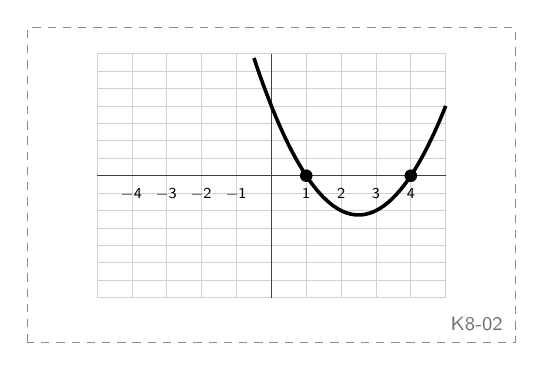
\begin{tikzpicture}
\useasboundingbox (0,0) rectangle (6.19,4.0);
\path[draw=black!18, line width=0.3pt] (0.881,0.57) -- (0.881,3.67);
\path[draw=black!18, line width=0.3pt] (1.324,0.57) -- (1.324,3.67);
\path[draw=black!18, line width=0.3pt] (1.766,0.57) -- (1.766,3.67);
\path[draw=black!18, line width=0.3pt] (2.209,0.57) -- (2.209,3.67);
\path[draw=black!18, line width=0.3pt] (2.652,0.57) -- (2.652,3.67);
\path[draw=black!18, line width=0.3pt] (3.095,0.57) -- (3.095,3.67);
\path[draw=black!18, line width=0.3pt] (3.538,0.57) -- (3.538,3.67);
\path[draw=black!18, line width=0.3pt] (3.981,0.57) -- (3.981,3.67);
\path[draw=black!18, line width=0.3pt] (4.424,0.57) -- (4.424,3.67);
\path[draw=black!18, line width=0.3pt] (4.866,0.57) -- (4.866,3.67);
\path[draw=black!18, line width=0.3pt] (5.309,0.57) -- (5.309,3.67);
\path[draw=black!18, line width=0.3pt] (0.881,0.57) -- (5.309,0.57);
\path[draw=black!18, line width=0.3pt] (0.881,0.791) -- (5.309,0.791);
\path[draw=black!18, line width=0.3pt] (0.881,1.013) -- (5.309,1.013);
\path[draw=black!18, line width=0.3pt] (0.881,1.234) -- (5.309,1.234);
\path[draw=black!18, line width=0.3pt] (0.881,1.456) -- (5.309,1.456);
\path[draw=black!18, line width=0.3pt] (0.881,1.677) -- (5.309,1.677);
\path[draw=black!18, line width=0.3pt] (0.881,1.899) -- (5.309,1.899);
\path[draw=black!18, line width=0.3pt] (0.881,2.12) -- (5.309,2.12);
\path[draw=black!18, line width=0.3pt] (0.881,2.341) -- (5.309,2.341);
\path[draw=black!18, line width=0.3pt] (0.881,2.563) -- (5.309,2.563);
\path[draw=black!18, line width=0.3pt] (0.881,2.784) -- (5.309,2.784);
\path[draw=black!18, line width=0.3pt] (0.881,3.006) -- (5.309,3.006);
\path[draw=black!18, line width=0.3pt] (0.881,3.227) -- (5.309,3.227);
\path[draw=black!18, line width=0.3pt] (0.881,3.449) -- (5.309,3.449);
\path[draw=black!18, line width=0.3pt] (0.881,3.67) -- (5.309,3.67);
\path[draw=black!75, line width=0.5pt] (0.881,2.12) -- (5.309,2.12);
\path[draw=black!75, line width=0.5pt] (3.095,0.57) -- (3.095,3.67);
\node[font=\sffamily\fontsize{5.5}{6}\selectfont, inner sep=0pt] at (1.324,1.899) {$-$4};
\node[font=\sffamily\fontsize{5.5}{6}\selectfont, inner sep=0pt] at (1.766,1.899) {$-$3};
\node[font=\sffamily\fontsize{5.5}{6}\selectfont, inner sep=0pt] at (2.209,1.899) {$-$2};
\node[font=\sffamily\fontsize{5.5}{6}\selectfont, inner sep=0pt] at (2.652,1.899) {$-$1};
\node[font=\sffamily\fontsize{5.5}{6}\selectfont, inner sep=0pt] at (3.538,1.899) {1};
\node[font=\sffamily\fontsize{5.5}{6}\selectfont, inner sep=0pt] at (3.981,1.899) {2};
\node[font=\sffamily\fontsize{5.5}{6}\selectfont, inner sep=0pt] at (4.424,1.899) {3};
\node[font=\sffamily\fontsize{5.5}{6}\selectfont, inner sep=0pt] at (4.866,1.899) {4};
\path[draw=black, line width=1.3pt] (2.874,3.615) -- (2.892,3.56) -- (2.91,3.505) -- (2.929,3.452) -- (2.947,3.399) -- (2.966,3.347) -- (2.984,3.296) -- (3.003,3.246) -- (3.021,3.196) -- (3.04,3.148) -- (3.058,3.1) -- (3.077,3.052) -- (3.095,3.006) -- (3.113,2.96) -- (3.132,2.915) -- (3.15,2.871) -- (3.169,2.827) -- (3.187,2.785) -- (3.206,2.743) -- (3.224,2.702) -- (3.243,2.661) -- (3.261,2.622) -- (3.28,2.583) -- (3.298,2.545) -- (3.316,2.508) -- (3.335,2.471) -- (3.353,2.435) -- (3.372,2.4) -- (3.39,2.366) -- (3.409,2.333) -- (3.427,2.3) -- (3.446,2.268) -- (3.464,2.237) -- (3.483,2.206) -- (3.501,2.177) -- (3.519,2.148) -- (3.538,2.12) -- (3.556,2.093) -- (3.575,2.066) -- (3.593,2.04) -- (3.612,2.015) -- (3.63,1.991) -- (3.649,1.968) -- (3.667,1.945) -- (3.685,1.923) -- (3.704,1.902) -- (3.722,1.882) -- (3.741,1.862) -- (3.759,1.843) -- (3.778,1.825) -- (3.796,1.808) -- (3.815,1.791) -- (3.833,1.776) -- (3.852,1.761) -- (3.87,1.746) -- (3.888,1.733) -- (3.907,1.72) -- (3.925,1.708) -- (3.944,1.697) -- (3.962,1.687) -- (3.981,1.677) -- (3.999,1.668) -- (4.018,1.66) -- (4.036,1.653) -- (4.055,1.646) -- (4.073,1.641) -- (4.091,1.636) -- (4.11,1.631) -- (4.128,1.628) -- (4.147,1.625) -- (4.165,1.623) -- (4.184,1.622) -- (4.202,1.622) -- (4.221,1.622) -- (4.239,1.623) -- (4.258,1.625) -- (4.276,1.628) -- (4.294,1.631) -- (4.313,1.636) -- (4.331,1.641) -- (4.35,1.646) -- (4.368,1.653) -- (4.387,1.66) -- (4.405,1.668) -- (4.424,1.677) -- (4.442,1.687) -- (4.46,1.697) -- (4.479,1.708) -- (4.497,1.72) -- (4.516,1.733) -- (4.534,1.746) -- (4.553,1.761) -- (4.571,1.776) -- (4.59,1.791) -- (4.608,1.808) -- (4.627,1.825) -- (4.645,1.843) -- (4.663,1.862) -- (4.682,1.882) -- (4.7,1.902) -- (4.719,1.923) -- (4.737,1.945) -- (4.756,1.968) -- (4.774,1.991) -- (4.793,2.015) -- (4.811,2.04) -- (4.83,2.066) -- (4.848,2.093) -- (4.866,2.12) -- (4.885,2.148) -- (4.903,2.177) -- (4.922,2.206) -- (4.94,2.237) -- (4.959,2.268) -- (4.977,2.3) -- (4.996,2.333) -- (5.014,2.366) -- (5.033,2.4) -- (5.051,2.435) -- (5.069,2.471) -- (5.088,2.508) -- (5.106,2.545) -- (5.125,2.583) -- (5.143,2.622) -- (5.162,2.661) -- (5.18,2.702) -- (5.199,2.743) -- (5.217,2.785) -- (5.235,2.827) -- (5.254,2.871) -- (5.272,2.915) -- (5.291,2.96) -- (5.309,3.006);
\path[fill=black] (3.538,2.12) circle[radius=0.08];
\path[fill=black] (4.866,2.12) circle[radius=0.08];
\draw[black!45, line width=0.4pt, dash pattern=on 3pt off 2.5pt] (0,0) rectangle (6.19,4.0);
\node[anchor=south east, font=\sffamily\scriptsize, text=black!55, inner sep=0pt] at (6.04,0.14) {K8-02};
\end{tikzpicture}%
\begin{tikzpicture}
\useasboundingbox (0,0) rectangle (6.19,4.0);
\node[text width=5.29cm, align=center, font=\Large] at (3.095,2.08) {$f(x) = (x + 2)(x - 2)$};
\draw[black!45, line width=0.4pt, dash pattern=on 3pt off 2.5pt] (0,0) rectangle (6.19,4.0);
\node[anchor=south east, font=\sffamily\scriptsize, text=black!55, inner sep=0pt] at (6.04,0.14) {K8-03};
\end{tikzpicture}%
\par\nointerlineskip
\noindent\begin{tikzpicture}
\useasboundingbox (0,0) rectangle (6.19,4.0);
\node[text width=5.29cm, align=center, font=\large] at (3.095,2.08) {Ett nullpunkt: $x = 3$};
\draw[black!45, line width=0.4pt, dash pattern=on 3pt off 2.5pt] (0,0) rectangle (6.19,4.0);
\node[anchor=south east, font=\sffamily\scriptsize, text=black!55, inner sep=0pt] at (6.04,0.14) {K8-04};
\end{tikzpicture}%
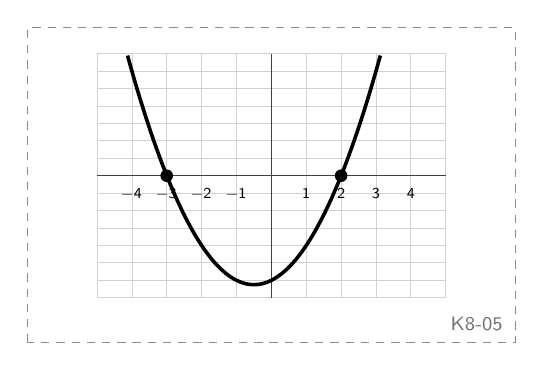
\begin{tikzpicture}
\useasboundingbox (0,0) rectangle (6.19,4.0);
\path[draw=black!18, line width=0.3pt] (0.881,0.57) -- (0.881,3.67);
\path[draw=black!18, line width=0.3pt] (1.324,0.57) -- (1.324,3.67);
\path[draw=black!18, line width=0.3pt] (1.766,0.57) -- (1.766,3.67);
\path[draw=black!18, line width=0.3pt] (2.209,0.57) -- (2.209,3.67);
\path[draw=black!18, line width=0.3pt] (2.652,0.57) -- (2.652,3.67);
\path[draw=black!18, line width=0.3pt] (3.095,0.57) -- (3.095,3.67);
\path[draw=black!18, line width=0.3pt] (3.538,0.57) -- (3.538,3.67);
\path[draw=black!18, line width=0.3pt] (3.981,0.57) -- (3.981,3.67);
\path[draw=black!18, line width=0.3pt] (4.424,0.57) -- (4.424,3.67);
\path[draw=black!18, line width=0.3pt] (4.866,0.57) -- (4.866,3.67);
\path[draw=black!18, line width=0.3pt] (5.309,0.57) -- (5.309,3.67);
\path[draw=black!18, line width=0.3pt] (0.881,0.57) -- (5.309,0.57);
\path[draw=black!18, line width=0.3pt] (0.881,0.791) -- (5.309,0.791);
\path[draw=black!18, line width=0.3pt] (0.881,1.013) -- (5.309,1.013);
\path[draw=black!18, line width=0.3pt] (0.881,1.234) -- (5.309,1.234);
\path[draw=black!18, line width=0.3pt] (0.881,1.456) -- (5.309,1.456);
\path[draw=black!18, line width=0.3pt] (0.881,1.677) -- (5.309,1.677);
\path[draw=black!18, line width=0.3pt] (0.881,1.899) -- (5.309,1.899);
\path[draw=black!18, line width=0.3pt] (0.881,2.12) -- (5.309,2.12);
\path[draw=black!18, line width=0.3pt] (0.881,2.341) -- (5.309,2.341);
\path[draw=black!18, line width=0.3pt] (0.881,2.563) -- (5.309,2.563);
\path[draw=black!18, line width=0.3pt] (0.881,2.784) -- (5.309,2.784);
\path[draw=black!18, line width=0.3pt] (0.881,3.006) -- (5.309,3.006);
\path[draw=black!18, line width=0.3pt] (0.881,3.227) -- (5.309,3.227);
\path[draw=black!18, line width=0.3pt] (0.881,3.449) -- (5.309,3.449);
\path[draw=black!18, line width=0.3pt] (0.881,3.67) -- (5.309,3.67);
\path[draw=black!75, line width=0.5pt] (0.881,2.12) -- (5.309,2.12);
\path[draw=black!75, line width=0.5pt] (3.095,0.57) -- (3.095,3.67);
\node[font=\sffamily\fontsize{5.5}{6}\selectfont, inner sep=0pt] at (1.324,1.899) {$-$4};
\node[font=\sffamily\fontsize{5.5}{6}\selectfont, inner sep=0pt] at (1.766,1.899) {$-$3};
\node[font=\sffamily\fontsize{5.5}{6}\selectfont, inner sep=0pt] at (2.209,1.899) {$-$2};
\node[font=\sffamily\fontsize{5.5}{6}\selectfont, inner sep=0pt] at (2.652,1.899) {$-$1};
\node[font=\sffamily\fontsize{5.5}{6}\selectfont, inner sep=0pt] at (3.538,1.899) {1};
\node[font=\sffamily\fontsize{5.5}{6}\selectfont, inner sep=0pt] at (3.981,1.899) {2};
\node[font=\sffamily\fontsize{5.5}{6}\selectfont, inner sep=0pt] at (4.424,1.899) {3};
\node[font=\sffamily\fontsize{5.5}{6}\selectfont, inner sep=0pt] at (4.866,1.899) {4};
\path[draw=black, line width=1.3pt] (1.268,3.646) -- (1.287,3.579) -- (1.305,3.514) -- (1.324,3.449) -- (1.342,3.384) -- (1.36,3.321) -- (1.379,3.258) -- (1.397,3.196) -- (1.416,3.135) -- (1.434,3.075) -- (1.453,3.015) -- (1.471,2.957) -- (1.49,2.898) -- (1.508,2.841) -- (1.527,2.785) -- (1.545,2.729) -- (1.563,2.674) -- (1.582,2.62) -- (1.6,2.566) -- (1.619,2.514) -- (1.637,2.462) -- (1.656,2.411) -- (1.674,2.36) -- (1.693,2.311) -- (1.711,2.262) -- (1.73,2.214) -- (1.748,2.167) -- (1.766,2.12) -- (1.785,2.074) -- (1.803,2.029) -- (1.822,1.985) -- (1.84,1.942) -- (1.859,1.899) -- (1.877,1.857) -- (1.896,1.816) -- (1.914,1.776) -- (1.933,1.736) -- (1.951,1.697) -- (1.969,1.659) -- (1.988,1.622) -- (2.006,1.585) -- (2.025,1.55) -- (2.043,1.515) -- (2.062,1.48) -- (2.08,1.447) -- (2.099,1.414) -- (2.117,1.382) -- (2.135,1.351) -- (2.154,1.321) -- (2.172,1.291) -- (2.191,1.262) -- (2.209,1.234) -- (2.228,1.207) -- (2.246,1.18) -- (2.265,1.155) -- (2.283,1.13) -- (2.302,1.106) -- (2.32,1.082) -- (2.338,1.059) -- (2.357,1.037) -- (2.375,1.016) -- (2.394,0.996) -- (2.412,0.976) -- (2.431,0.958) -- (2.449,0.939) -- (2.468,0.922) -- (2.486,0.906) -- (2.505,0.89) -- (2.523,0.875) -- (2.541,0.861) -- (2.56,0.847) -- (2.578,0.834) -- (2.597,0.823) -- (2.615,0.811) -- (2.634,0.801) -- (2.652,0.791) -- (2.671,0.783) -- (2.689,0.775) -- (2.708,0.767) -- (2.726,0.761) -- (2.744,0.755) -- (2.763,0.75) -- (2.781,0.746) -- (2.8,0.742) -- (2.818,0.74) -- (2.837,0.738) -- (2.855,0.736) -- (2.874,0.736) -- (2.892,0.736) -- (2.91,0.738) -- (2.929,0.74) -- (2.947,0.742) -- (2.966,0.746) -- (2.984,0.75) -- (3.003,0.755) -- (3.021,0.761) -- (3.04,0.767) -- (3.058,0.775) -- (3.077,0.783) -- (3.095,0.791) -- (3.113,0.801) -- (3.132,0.811) -- (3.15,0.823) -- (3.169,0.834) -- (3.187,0.847) -- (3.206,0.861) -- (3.224,0.875) -- (3.243,0.89) -- (3.261,0.906) -- (3.28,0.922) -- (3.298,0.939) -- (3.316,0.958) -- (3.335,0.976) -- (3.353,0.996) -- (3.372,1.016) -- (3.39,1.037) -- (3.409,1.059) -- (3.427,1.082) -- (3.446,1.106) -- (3.464,1.13) -- (3.483,1.155) -- (3.501,1.18) -- (3.519,1.207) -- (3.538,1.234) -- (3.556,1.262) -- (3.575,1.291) -- (3.593,1.321) -- (3.612,1.351) -- (3.63,1.382) -- (3.649,1.414) -- (3.667,1.447) -- (3.685,1.48) -- (3.704,1.515) -- (3.722,1.55) -- (3.741,1.585) -- (3.759,1.622) -- (3.778,1.659) -- (3.796,1.697) -- (3.815,1.736) -- (3.833,1.776) -- (3.852,1.816) -- (3.87,1.857) -- (3.888,1.899) -- (3.907,1.942) -- (3.925,1.985) -- (3.944,2.029) -- (3.962,2.074) -- (3.981,2.12) -- (3.999,2.167) -- (4.018,2.214) -- (4.036,2.262) -- (4.055,2.311) -- (4.073,2.36) -- (4.091,2.411) -- (4.11,2.462) -- (4.128,2.514) -- (4.147,2.566) -- (4.165,2.62) -- (4.184,2.674) -- (4.202,2.729) -- (4.221,2.785) -- (4.239,2.841) -- (4.258,2.898) -- (4.276,2.957) -- (4.294,3.015) -- (4.313,3.075) -- (4.331,3.135) -- (4.35,3.196) -- (4.368,3.258) -- (4.387,3.321) -- (4.405,3.384) -- (4.424,3.449) -- (4.442,3.514) -- (4.46,3.579) -- (4.479,3.646);
\path[fill=black] (3.981,2.12) circle[radius=0.08];
\path[fill=black] (1.766,2.12) circle[radius=0.08];
\draw[black!45, line width=0.4pt, dash pattern=on 3pt off 2.5pt] (0,0) rectangle (6.19,4.0);
\node[anchor=south east, font=\sffamily\scriptsize, text=black!55, inner sep=0pt] at (6.04,0.14) {K8-05};
\end{tikzpicture}%
\begin{tikzpicture}
\useasboundingbox (0,0) rectangle (6.19,4.0);
\node[text width=5.29cm, align=center, font=\Large] at (3.095,2.08) {$f(x) = (x + 3)(x - 2)$};
\draw[black!45, line width=0.4pt, dash pattern=on 3pt off 2.5pt] (0,0) rectangle (6.19,4.0);
\node[anchor=south east, font=\sffamily\scriptsize, text=black!55, inner sep=0pt] at (6.04,0.14) {K8-06};
\end{tikzpicture}%
\par\nointerlineskip
\noindent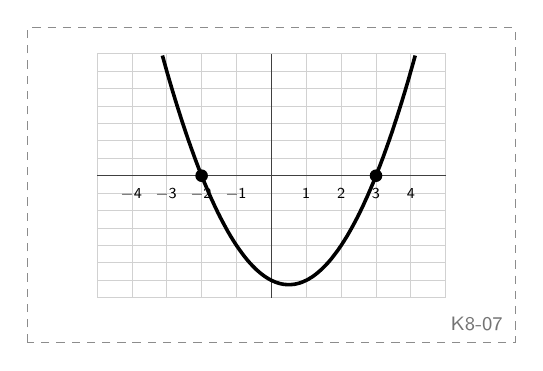
\begin{tikzpicture}
\useasboundingbox (0,0) rectangle (6.19,4.0);
\path[draw=black!18, line width=0.3pt] (0.881,0.57) -- (0.881,3.67);
\path[draw=black!18, line width=0.3pt] (1.324,0.57) -- (1.324,3.67);
\path[draw=black!18, line width=0.3pt] (1.766,0.57) -- (1.766,3.67);
\path[draw=black!18, line width=0.3pt] (2.209,0.57) -- (2.209,3.67);
\path[draw=black!18, line width=0.3pt] (2.652,0.57) -- (2.652,3.67);
\path[draw=black!18, line width=0.3pt] (3.095,0.57) -- (3.095,3.67);
\path[draw=black!18, line width=0.3pt] (3.538,0.57) -- (3.538,3.67);
\path[draw=black!18, line width=0.3pt] (3.981,0.57) -- (3.981,3.67);
\path[draw=black!18, line width=0.3pt] (4.424,0.57) -- (4.424,3.67);
\path[draw=black!18, line width=0.3pt] (4.866,0.57) -- (4.866,3.67);
\path[draw=black!18, line width=0.3pt] (5.309,0.57) -- (5.309,3.67);
\path[draw=black!18, line width=0.3pt] (0.881,0.57) -- (5.309,0.57);
\path[draw=black!18, line width=0.3pt] (0.881,0.791) -- (5.309,0.791);
\path[draw=black!18, line width=0.3pt] (0.881,1.013) -- (5.309,1.013);
\path[draw=black!18, line width=0.3pt] (0.881,1.234) -- (5.309,1.234);
\path[draw=black!18, line width=0.3pt] (0.881,1.456) -- (5.309,1.456);
\path[draw=black!18, line width=0.3pt] (0.881,1.677) -- (5.309,1.677);
\path[draw=black!18, line width=0.3pt] (0.881,1.899) -- (5.309,1.899);
\path[draw=black!18, line width=0.3pt] (0.881,2.12) -- (5.309,2.12);
\path[draw=black!18, line width=0.3pt] (0.881,2.341) -- (5.309,2.341);
\path[draw=black!18, line width=0.3pt] (0.881,2.563) -- (5.309,2.563);
\path[draw=black!18, line width=0.3pt] (0.881,2.784) -- (5.309,2.784);
\path[draw=black!18, line width=0.3pt] (0.881,3.006) -- (5.309,3.006);
\path[draw=black!18, line width=0.3pt] (0.881,3.227) -- (5.309,3.227);
\path[draw=black!18, line width=0.3pt] (0.881,3.449) -- (5.309,3.449);
\path[draw=black!18, line width=0.3pt] (0.881,3.67) -- (5.309,3.67);
\path[draw=black!75, line width=0.5pt] (0.881,2.12) -- (5.309,2.12);
\path[draw=black!75, line width=0.5pt] (3.095,0.57) -- (3.095,3.67);
\node[font=\sffamily\fontsize{5.5}{6}\selectfont, inner sep=0pt] at (1.324,1.899) {$-$4};
\node[font=\sffamily\fontsize{5.5}{6}\selectfont, inner sep=0pt] at (1.766,1.899) {$-$3};
\node[font=\sffamily\fontsize{5.5}{6}\selectfont, inner sep=0pt] at (2.209,1.899) {$-$2};
\node[font=\sffamily\fontsize{5.5}{6}\selectfont, inner sep=0pt] at (2.652,1.899) {$-$1};
\node[font=\sffamily\fontsize{5.5}{6}\selectfont, inner sep=0pt] at (3.538,1.899) {1};
\node[font=\sffamily\fontsize{5.5}{6}\selectfont, inner sep=0pt] at (3.981,1.899) {2};
\node[font=\sffamily\fontsize{5.5}{6}\selectfont, inner sep=0pt] at (4.424,1.899) {3};
\node[font=\sffamily\fontsize{5.5}{6}\selectfont, inner sep=0pt] at (4.866,1.899) {4};
\path[draw=black, line width=1.3pt] (1.711,3.646) -- (1.73,3.579) -- (1.748,3.514) -- (1.766,3.449) -- (1.785,3.384) -- (1.803,3.321) -- (1.822,3.258) -- (1.84,3.196) -- (1.859,3.135) -- (1.877,3.075) -- (1.896,3.015) -- (1.914,2.957) -- (1.933,2.898) -- (1.951,2.841) -- (1.969,2.785) -- (1.988,2.729) -- (2.006,2.674) -- (2.025,2.62) -- (2.043,2.566) -- (2.062,2.514) -- (2.08,2.462) -- (2.099,2.411) -- (2.117,2.36) -- (2.135,2.311) -- (2.154,2.262) -- (2.172,2.214) -- (2.191,2.167) -- (2.209,2.12) -- (2.228,2.074) -- (2.246,2.029) -- (2.265,1.985) -- (2.283,1.942) -- (2.302,1.899) -- (2.32,1.857) -- (2.338,1.816) -- (2.357,1.776) -- (2.375,1.736) -- (2.394,1.697) -- (2.412,1.659) -- (2.431,1.622) -- (2.449,1.585) -- (2.468,1.55) -- (2.486,1.515) -- (2.505,1.48) -- (2.523,1.447) -- (2.541,1.414) -- (2.56,1.382) -- (2.578,1.351) -- (2.597,1.321) -- (2.615,1.291) -- (2.634,1.262) -- (2.652,1.234) -- (2.671,1.207) -- (2.689,1.18) -- (2.708,1.155) -- (2.726,1.13) -- (2.744,1.106) -- (2.763,1.082) -- (2.781,1.059) -- (2.8,1.037) -- (2.818,1.016) -- (2.837,0.996) -- (2.855,0.976) -- (2.874,0.958) -- (2.892,0.939) -- (2.91,0.922) -- (2.929,0.906) -- (2.947,0.89) -- (2.966,0.875) -- (2.984,0.861) -- (3.003,0.847) -- (3.021,0.834) -- (3.04,0.823) -- (3.058,0.811) -- (3.077,0.801) -- (3.095,0.791) -- (3.113,0.783) -- (3.132,0.775) -- (3.15,0.767) -- (3.169,0.761) -- (3.187,0.755) -- (3.206,0.75) -- (3.224,0.746) -- (3.243,0.742) -- (3.261,0.74) -- (3.28,0.738) -- (3.298,0.736) -- (3.316,0.736) -- (3.335,0.736) -- (3.353,0.738) -- (3.372,0.74) -- (3.39,0.742) -- (3.409,0.746) -- (3.427,0.75) -- (3.446,0.755) -- (3.464,0.761) -- (3.483,0.767) -- (3.501,0.775) -- (3.519,0.783) -- (3.538,0.791) -- (3.556,0.801) -- (3.575,0.811) -- (3.593,0.823) -- (3.612,0.834) -- (3.63,0.847) -- (3.649,0.861) -- (3.667,0.875) -- (3.685,0.89) -- (3.704,0.906) -- (3.722,0.922) -- (3.741,0.939) -- (3.759,0.958) -- (3.778,0.976) -- (3.796,0.996) -- (3.815,1.016) -- (3.833,1.037) -- (3.852,1.059) -- (3.87,1.082) -- (3.888,1.106) -- (3.907,1.13) -- (3.925,1.155) -- (3.944,1.18) -- (3.962,1.207) -- (3.981,1.234) -- (3.999,1.262) -- (4.018,1.291) -- (4.036,1.321) -- (4.055,1.351) -- (4.073,1.382) -- (4.091,1.414) -- (4.11,1.447) -- (4.128,1.48) -- (4.147,1.515) -- (4.165,1.55) -- (4.184,1.585) -- (4.202,1.622) -- (4.221,1.659) -- (4.239,1.697) -- (4.258,1.736) -- (4.276,1.776) -- (4.294,1.816) -- (4.313,1.857) -- (4.331,1.899) -- (4.35,1.942) -- (4.368,1.985) -- (4.387,2.029) -- (4.405,2.074) -- (4.424,2.12) -- (4.442,2.167) -- (4.46,2.214) -- (4.479,2.262) -- (4.497,2.311) -- (4.516,2.36) -- (4.534,2.411) -- (4.553,2.462) -- (4.571,2.514) -- (4.59,2.566) -- (4.608,2.62) -- (4.627,2.674) -- (4.645,2.729) -- (4.663,2.785) -- (4.682,2.841) -- (4.7,2.898) -- (4.719,2.957) -- (4.737,3.015) -- (4.756,3.075) -- (4.774,3.135) -- (4.793,3.196) -- (4.811,3.258) -- (4.83,3.321) -- (4.848,3.384) -- (4.866,3.449) -- (4.885,3.514) -- (4.903,3.579) -- (4.922,3.646);
\path[fill=black] (4.424,2.12) circle[radius=0.08];
\path[fill=black] (2.209,2.12) circle[radius=0.08];
\draw[black!45, line width=0.4pt, dash pattern=on 3pt off 2.5pt] (0,0) rectangle (6.19,4.0);
\node[anchor=south east, font=\sffamily\scriptsize, text=black!55, inner sep=0pt] at (6.04,0.14) {K8-07};
\end{tikzpicture}%
\begin{tikzpicture}
\useasboundingbox (0,0) rectangle (6.19,4.0);
\node[text width=5.29cm, align=center, font=\large] at (3.095,2.08) {Nullpunkter: $x = -3$ og $x = 2$};
\draw[black!45, line width=0.4pt, dash pattern=on 3pt off 2.5pt] (0,0) rectangle (6.19,4.0);
\node[anchor=south east, font=\sffamily\scriptsize, text=black!55, inner sep=0pt] at (6.04,0.14) {K8-08};
\end{tikzpicture}%
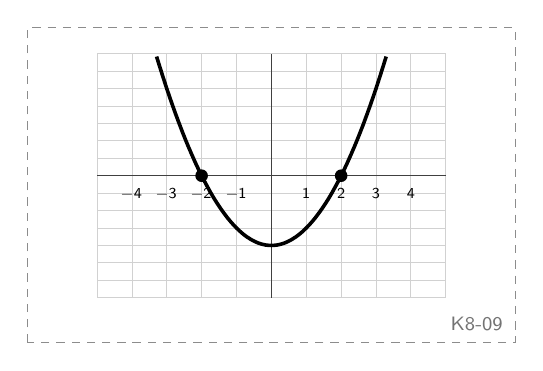
\begin{tikzpicture}
\useasboundingbox (0,0) rectangle (6.19,4.0);
\path[draw=black!18, line width=0.3pt] (0.881,0.57) -- (0.881,3.67);
\path[draw=black!18, line width=0.3pt] (1.324,0.57) -- (1.324,3.67);
\path[draw=black!18, line width=0.3pt] (1.766,0.57) -- (1.766,3.67);
\path[draw=black!18, line width=0.3pt] (2.209,0.57) -- (2.209,3.67);
\path[draw=black!18, line width=0.3pt] (2.652,0.57) -- (2.652,3.67);
\path[draw=black!18, line width=0.3pt] (3.095,0.57) -- (3.095,3.67);
\path[draw=black!18, line width=0.3pt] (3.538,0.57) -- (3.538,3.67);
\path[draw=black!18, line width=0.3pt] (3.981,0.57) -- (3.981,3.67);
\path[draw=black!18, line width=0.3pt] (4.424,0.57) -- (4.424,3.67);
\path[draw=black!18, line width=0.3pt] (4.866,0.57) -- (4.866,3.67);
\path[draw=black!18, line width=0.3pt] (5.309,0.57) -- (5.309,3.67);
\path[draw=black!18, line width=0.3pt] (0.881,0.57) -- (5.309,0.57);
\path[draw=black!18, line width=0.3pt] (0.881,0.791) -- (5.309,0.791);
\path[draw=black!18, line width=0.3pt] (0.881,1.013) -- (5.309,1.013);
\path[draw=black!18, line width=0.3pt] (0.881,1.234) -- (5.309,1.234);
\path[draw=black!18, line width=0.3pt] (0.881,1.456) -- (5.309,1.456);
\path[draw=black!18, line width=0.3pt] (0.881,1.677) -- (5.309,1.677);
\path[draw=black!18, line width=0.3pt] (0.881,1.899) -- (5.309,1.899);
\path[draw=black!18, line width=0.3pt] (0.881,2.12) -- (5.309,2.12);
\path[draw=black!18, line width=0.3pt] (0.881,2.341) -- (5.309,2.341);
\path[draw=black!18, line width=0.3pt] (0.881,2.563) -- (5.309,2.563);
\path[draw=black!18, line width=0.3pt] (0.881,2.784) -- (5.309,2.784);
\path[draw=black!18, line width=0.3pt] (0.881,3.006) -- (5.309,3.006);
\path[draw=black!18, line width=0.3pt] (0.881,3.227) -- (5.309,3.227);
\path[draw=black!18, line width=0.3pt] (0.881,3.449) -- (5.309,3.449);
\path[draw=black!18, line width=0.3pt] (0.881,3.67) -- (5.309,3.67);
\path[draw=black!75, line width=0.5pt] (0.881,2.12) -- (5.309,2.12);
\path[draw=black!75, line width=0.5pt] (3.095,0.57) -- (3.095,3.67);
\node[font=\sffamily\fontsize{5.5}{6}\selectfont, inner sep=0pt] at (1.324,1.899) {$-$4};
\node[font=\sffamily\fontsize{5.5}{6}\selectfont, inner sep=0pt] at (1.766,1.899) {$-$3};
\node[font=\sffamily\fontsize{5.5}{6}\selectfont, inner sep=0pt] at (2.209,1.899) {$-$2};
\node[font=\sffamily\fontsize{5.5}{6}\selectfont, inner sep=0pt] at (2.652,1.899) {$-$1};
\node[font=\sffamily\fontsize{5.5}{6}\selectfont, inner sep=0pt] at (3.538,1.899) {1};
\node[font=\sffamily\fontsize{5.5}{6}\selectfont, inner sep=0pt] at (3.981,1.899) {2};
\node[font=\sffamily\fontsize{5.5}{6}\selectfont, inner sep=0pt] at (4.424,1.899) {3};
\node[font=\sffamily\fontsize{5.5}{6}\selectfont, inner sep=0pt] at (4.866,1.899) {4};
\path[draw=black, line width=1.3pt] (1.637,3.633) -- (1.656,3.573) -- (1.674,3.514) -- (1.693,3.455) -- (1.711,3.397) -- (1.73,3.339) -- (1.748,3.283) -- (1.766,3.227) -- (1.785,3.172) -- (1.803,3.118) -- (1.822,3.065) -- (1.84,3.012) -- (1.859,2.96) -- (1.877,2.909) -- (1.896,2.858) -- (1.914,2.809) -- (1.933,2.76) -- (1.951,2.712) -- (1.969,2.665) -- (1.988,2.618) -- (2.006,2.572) -- (2.025,2.527) -- (2.043,2.483) -- (2.062,2.44) -- (2.08,2.397) -- (2.099,2.355) -- (2.117,2.314) -- (2.135,2.274) -- (2.154,2.234) -- (2.172,2.195) -- (2.191,2.157) -- (2.209,2.12) -- (2.228,2.083) -- (2.246,2.048) -- (2.265,2.013) -- (2.283,1.979) -- (2.302,1.945) -- (2.32,1.912) -- (2.338,1.881) -- (2.357,1.849) -- (2.375,1.819) -- (2.394,1.789) -- (2.412,1.761) -- (2.431,1.733) -- (2.449,1.705) -- (2.468,1.679) -- (2.486,1.653) -- (2.505,1.628) -- (2.523,1.604) -- (2.541,1.58) -- (2.56,1.558) -- (2.578,1.536) -- (2.597,1.515) -- (2.615,1.494) -- (2.634,1.475) -- (2.652,1.456) -- (2.671,1.438) -- (2.689,1.42) -- (2.708,1.404) -- (2.726,1.388) -- (2.744,1.373) -- (2.763,1.359) -- (2.781,1.345) -- (2.8,1.333) -- (2.818,1.321) -- (2.837,1.31) -- (2.855,1.299) -- (2.874,1.29) -- (2.892,1.281) -- (2.91,1.273) -- (2.929,1.265) -- (2.947,1.259) -- (2.966,1.253) -- (2.984,1.248) -- (3.003,1.244) -- (3.021,1.24) -- (3.04,1.238) -- (3.058,1.236) -- (3.077,1.235) -- (3.095,1.234) -- (3.113,1.235) -- (3.132,1.236) -- (3.15,1.238) -- (3.169,1.24) -- (3.187,1.244) -- (3.206,1.248) -- (3.224,1.253) -- (3.243,1.259) -- (3.261,1.265) -- (3.28,1.273) -- (3.298,1.281) -- (3.316,1.29) -- (3.335,1.299) -- (3.353,1.31) -- (3.372,1.321) -- (3.39,1.333) -- (3.409,1.345) -- (3.427,1.359) -- (3.446,1.373) -- (3.464,1.388) -- (3.483,1.404) -- (3.501,1.42) -- (3.519,1.438) -- (3.538,1.456) -- (3.556,1.475) -- (3.575,1.494) -- (3.593,1.515) -- (3.612,1.536) -- (3.63,1.558) -- (3.649,1.58) -- (3.667,1.604) -- (3.685,1.628) -- (3.704,1.653) -- (3.722,1.679) -- (3.741,1.705) -- (3.759,1.733) -- (3.778,1.761) -- (3.796,1.789) -- (3.815,1.819) -- (3.833,1.849) -- (3.852,1.881) -- (3.87,1.912) -- (3.888,1.945) -- (3.907,1.979) -- (3.925,2.013) -- (3.944,2.048) -- (3.962,2.083) -- (3.981,2.12) -- (3.999,2.157) -- (4.018,2.195) -- (4.036,2.234) -- (4.055,2.274) -- (4.073,2.314) -- (4.091,2.355) -- (4.11,2.397) -- (4.128,2.44) -- (4.147,2.483) -- (4.165,2.527) -- (4.184,2.572) -- (4.202,2.618) -- (4.221,2.665) -- (4.239,2.712) -- (4.258,2.76) -- (4.276,2.809) -- (4.294,2.858) -- (4.313,2.909) -- (4.331,2.96) -- (4.35,3.012) -- (4.368,3.065) -- (4.387,3.118) -- (4.405,3.172) -- (4.424,3.227) -- (4.442,3.283) -- (4.46,3.339) -- (4.479,3.397) -- (4.497,3.455) -- (4.516,3.514) -- (4.534,3.573) -- (4.553,3.633);
\path[fill=black] (3.981,2.12) circle[radius=0.08];
\path[fill=black] (2.209,2.12) circle[radius=0.08];
\draw[black!45, line width=0.4pt, dash pattern=on 3pt off 2.5pt] (0,0) rectangle (6.19,4.0);
\node[anchor=south east, font=\sffamily\scriptsize, text=black!55, inner sep=0pt] at (6.04,0.14) {K8-09};
\end{tikzpicture}%
\par\nointerlineskip
\noindent\begin{tikzpicture}
\useasboundingbox (0,0) rectangle (6.19,4.0);
\node[text width=5.29cm, align=center, font=\Large] at (3.095,2.08) {$f(x) = x^2 - 4$};
\draw[black!45, line width=0.4pt, dash pattern=on 3pt off 2.5pt] (0,0) rectangle (6.19,4.0);
\node[anchor=south east, font=\sffamily\scriptsize, text=black!55, inner sep=0pt] at (6.04,0.14) {K8-10};
\end{tikzpicture}%
\begin{tikzpicture}
\useasboundingbox (0,0) rectangle (6.19,4.0);
\node[text width=5.29cm, align=center, font=\Large] at (3.095,2.08) {$f(x) = x^2 - 3x$};
\draw[black!45, line width=0.4pt, dash pattern=on 3pt off 2.5pt] (0,0) rectangle (6.19,4.0);
\node[anchor=south east, font=\sffamily\scriptsize, text=black!55, inner sep=0pt] at (6.04,0.14) {K8-11};
\end{tikzpicture}%
\begin{tikzpicture}
\useasboundingbox (0,0) rectangle (6.19,4.0);
\node[text width=5.29cm, align=center, font=\large] at (3.095,2.08) {Nullpunkter: $x = 0$ og $x = 3$};
\draw[black!45, line width=0.4pt, dash pattern=on 3pt off 2.5pt] (0,0) rectangle (6.19,4.0);
\node[anchor=south east, font=\sffamily\scriptsize, text=black!55, inner sep=0pt] at (6.04,0.14) {K8-12};
\end{tikzpicture}%
\par\nointerlineskip
\noindent\begin{tikzpicture}
\useasboundingbox (0,0) rectangle (6.19,4.0);
\node[text width=5.29cm, align=center, font=\Large] at (3.095,2.08) {$f(x) = x^2 + 5x + 4$};
\draw[black!45, line width=0.4pt, dash pattern=on 3pt off 2.5pt] (0,0) rectangle (6.19,4.0);
\node[anchor=south east, font=\sffamily\scriptsize, text=black!55, inner sep=0pt] at (6.04,0.14) {K8-13};
\end{tikzpicture}%
\begin{tikzpicture}
\useasboundingbox (0,0) rectangle (6.19,4.0);
\node[text width=5.29cm, align=center, font=\large] at (3.095,2.08) {Nullpunkter: $x = -2$ og $x = 3$};
\draw[black!45, line width=0.4pt, dash pattern=on 3pt off 2.5pt] (0,0) rectangle (6.19,4.0);
\node[anchor=south east, font=\sffamily\scriptsize, text=black!55, inner sep=0pt] at (6.04,0.14) {K8-14};
\end{tikzpicture}%
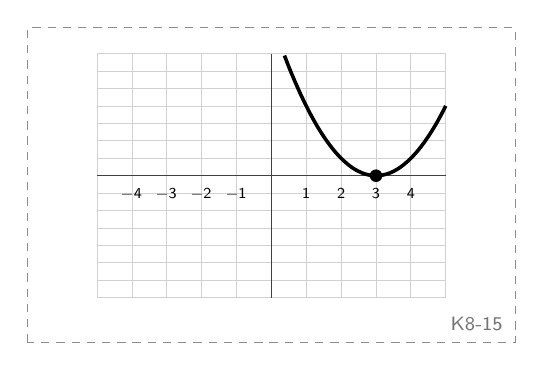
\begin{tikzpicture}
\useasboundingbox (0,0) rectangle (6.19,4.0);
\path[draw=black!18, line width=0.3pt] (0.881,0.57) -- (0.881,3.67);
\path[draw=black!18, line width=0.3pt] (1.324,0.57) -- (1.324,3.67);
\path[draw=black!18, line width=0.3pt] (1.766,0.57) -- (1.766,3.67);
\path[draw=black!18, line width=0.3pt] (2.209,0.57) -- (2.209,3.67);
\path[draw=black!18, line width=0.3pt] (2.652,0.57) -- (2.652,3.67);
\path[draw=black!18, line width=0.3pt] (3.095,0.57) -- (3.095,3.67);
\path[draw=black!18, line width=0.3pt] (3.538,0.57) -- (3.538,3.67);
\path[draw=black!18, line width=0.3pt] (3.981,0.57) -- (3.981,3.67);
\path[draw=black!18, line width=0.3pt] (4.424,0.57) -- (4.424,3.67);
\path[draw=black!18, line width=0.3pt] (4.866,0.57) -- (4.866,3.67);
\path[draw=black!18, line width=0.3pt] (5.309,0.57) -- (5.309,3.67);
\path[draw=black!18, line width=0.3pt] (0.881,0.57) -- (5.309,0.57);
\path[draw=black!18, line width=0.3pt] (0.881,0.791) -- (5.309,0.791);
\path[draw=black!18, line width=0.3pt] (0.881,1.013) -- (5.309,1.013);
\path[draw=black!18, line width=0.3pt] (0.881,1.234) -- (5.309,1.234);
\path[draw=black!18, line width=0.3pt] (0.881,1.456) -- (5.309,1.456);
\path[draw=black!18, line width=0.3pt] (0.881,1.677) -- (5.309,1.677);
\path[draw=black!18, line width=0.3pt] (0.881,1.899) -- (5.309,1.899);
\path[draw=black!18, line width=0.3pt] (0.881,2.12) -- (5.309,2.12);
\path[draw=black!18, line width=0.3pt] (0.881,2.341) -- (5.309,2.341);
\path[draw=black!18, line width=0.3pt] (0.881,2.563) -- (5.309,2.563);
\path[draw=black!18, line width=0.3pt] (0.881,2.784) -- (5.309,2.784);
\path[draw=black!18, line width=0.3pt] (0.881,3.006) -- (5.309,3.006);
\path[draw=black!18, line width=0.3pt] (0.881,3.227) -- (5.309,3.227);
\path[draw=black!18, line width=0.3pt] (0.881,3.449) -- (5.309,3.449);
\path[draw=black!18, line width=0.3pt] (0.881,3.67) -- (5.309,3.67);
\path[draw=black!75, line width=0.5pt] (0.881,2.12) -- (5.309,2.12);
\path[draw=black!75, line width=0.5pt] (3.095,0.57) -- (3.095,3.67);
\node[font=\sffamily\fontsize{5.5}{6}\selectfont, inner sep=0pt] at (1.324,1.899) {$-$4};
\node[font=\sffamily\fontsize{5.5}{6}\selectfont, inner sep=0pt] at (1.766,1.899) {$-$3};
\node[font=\sffamily\fontsize{5.5}{6}\selectfont, inner sep=0pt] at (2.209,1.899) {$-$2};
\node[font=\sffamily\fontsize{5.5}{6}\selectfont, inner sep=0pt] at (2.652,1.899) {$-$1};
\node[font=\sffamily\fontsize{5.5}{6}\selectfont, inner sep=0pt] at (3.538,1.899) {1};
\node[font=\sffamily\fontsize{5.5}{6}\selectfont, inner sep=0pt] at (3.981,1.899) {2};
\node[font=\sffamily\fontsize{5.5}{6}\selectfont, inner sep=0pt] at (4.424,1.899) {3};
\node[font=\sffamily\fontsize{5.5}{6}\selectfont, inner sep=0pt] at (4.866,1.899) {4};
\path[draw=black, line width=1.3pt] (3.261,3.646) -- (3.28,3.598) -- (3.298,3.55) -- (3.316,3.504) -- (3.335,3.458) -- (3.353,3.413) -- (3.372,3.369) -- (3.39,3.326) -- (3.409,3.283) -- (3.427,3.241) -- (3.446,3.2) -- (3.464,3.159) -- (3.483,3.12) -- (3.501,3.081) -- (3.519,3.043) -- (3.538,3.006) -- (3.556,2.969) -- (3.575,2.933) -- (3.593,2.898) -- (3.612,2.864) -- (3.63,2.831) -- (3.649,2.798) -- (3.667,2.766) -- (3.685,2.735) -- (3.704,2.705) -- (3.722,2.675) -- (3.741,2.646) -- (3.759,2.618) -- (3.778,2.591) -- (3.796,2.564) -- (3.815,2.539) -- (3.833,2.514) -- (3.852,2.489) -- (3.87,2.466) -- (3.888,2.443) -- (3.907,2.421) -- (3.925,2.4) -- (3.944,2.38) -- (3.962,2.36) -- (3.981,2.341) -- (3.999,2.323) -- (4.018,2.306) -- (4.036,2.29) -- (4.055,2.274) -- (4.073,2.259) -- (4.091,2.245) -- (4.11,2.231) -- (4.128,2.218) -- (4.147,2.206) -- (4.165,2.195) -- (4.184,2.185) -- (4.202,2.175) -- (4.221,2.167) -- (4.239,2.158) -- (4.258,2.151) -- (4.276,2.145) -- (4.294,2.139) -- (4.313,2.134) -- (4.331,2.13) -- (4.35,2.126) -- (4.368,2.123) -- (4.387,2.122) -- (4.405,2.12) -- (4.424,2.12) -- (4.442,2.12) -- (4.46,2.122) -- (4.479,2.123) -- (4.497,2.126) -- (4.516,2.13) -- (4.534,2.134) -- (4.553,2.139) -- (4.571,2.145) -- (4.59,2.151) -- (4.608,2.158) -- (4.627,2.167) -- (4.645,2.175) -- (4.663,2.185) -- (4.682,2.195) -- (4.7,2.206) -- (4.719,2.218) -- (4.737,2.231) -- (4.756,2.245) -- (4.774,2.259) -- (4.793,2.274) -- (4.811,2.29) -- (4.83,2.306) -- (4.848,2.323) -- (4.866,2.341) -- (4.885,2.36) -- (4.903,2.38) -- (4.922,2.4) -- (4.94,2.421) -- (4.959,2.443) -- (4.977,2.466) -- (4.996,2.489) -- (5.014,2.514) -- (5.033,2.539) -- (5.051,2.564) -- (5.069,2.591) -- (5.088,2.618) -- (5.106,2.646) -- (5.125,2.675) -- (5.143,2.705) -- (5.162,2.735) -- (5.18,2.766) -- (5.199,2.798) -- (5.217,2.831) -- (5.235,2.864) -- (5.254,2.898) -- (5.272,2.933) -- (5.291,2.969) -- (5.309,3.006);
\path[fill=black] (4.424,2.12) circle[radius=0.08];
\draw[black!45, line width=0.4pt, dash pattern=on 3pt off 2.5pt] (0,0) rectangle (6.19,4.0);
\node[anchor=south east, font=\sffamily\scriptsize, text=black!55, inner sep=0pt] at (6.04,0.14) {K8-15};
\end{tikzpicture}%
\par\nointerlineskip
\noindent\begin{tikzpicture}
\useasboundingbox (0,0) rectangle (6.19,4.0);
\node[text width=5.29cm, align=center, font=\Large] at (3.095,2.08) {$f(x) = (x + 2)(x - 3)$};
\draw[black!45, line width=0.4pt, dash pattern=on 3pt off 2.5pt] (0,0) rectangle (6.19,4.0);
\node[anchor=south east, font=\sffamily\scriptsize, text=black!55, inner sep=0pt] at (6.04,0.14) {K8-16};
\end{tikzpicture}%
\begin{tikzpicture}
\useasboundingbox (0,0) rectangle (6.19,4.0);
\node[text width=5.29cm, align=center, font=\large] at (3.095,2.08) {Nullpunkter: $x = -4$ og $x = -1$};
\draw[black!45, line width=0.4pt, dash pattern=on 3pt off 2.5pt] (0,0) rectangle (6.19,4.0);
\node[anchor=south east, font=\sffamily\scriptsize, text=black!55, inner sep=0pt] at (6.04,0.14) {K8-17};
\end{tikzpicture}%
\begin{tikzpicture}
\useasboundingbox (0,0) rectangle (6.19,4.0);
\node[text width=5.29cm, align=center, font=\large] at (3.095,2.08) {Nullpunkter: $x = -2$ og $x = 2$};
\draw[black!45, line width=0.4pt, dash pattern=on 3pt off 2.5pt] (0,0) rectangle (6.19,4.0);
\node[anchor=south east, font=\sffamily\scriptsize, text=black!55, inner sep=0pt] at (6.04,0.14) {K8-18};
\end{tikzpicture}%
\par\nointerlineskip
\noindent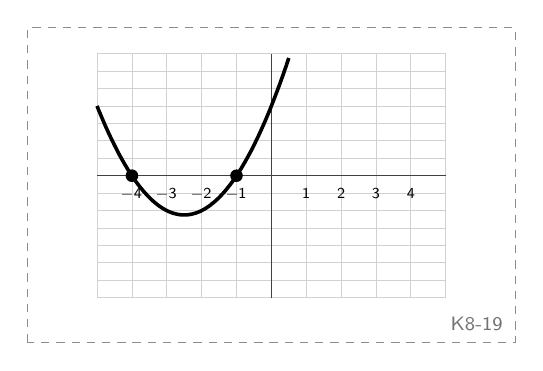
\begin{tikzpicture}
\useasboundingbox (0,0) rectangle (6.19,4.0);
\path[draw=black!18, line width=0.3pt] (0.881,0.57) -- (0.881,3.67);
\path[draw=black!18, line width=0.3pt] (1.324,0.57) -- (1.324,3.67);
\path[draw=black!18, line width=0.3pt] (1.766,0.57) -- (1.766,3.67);
\path[draw=black!18, line width=0.3pt] (2.209,0.57) -- (2.209,3.67);
\path[draw=black!18, line width=0.3pt] (2.652,0.57) -- (2.652,3.67);
\path[draw=black!18, line width=0.3pt] (3.095,0.57) -- (3.095,3.67);
\path[draw=black!18, line width=0.3pt] (3.538,0.57) -- (3.538,3.67);
\path[draw=black!18, line width=0.3pt] (3.981,0.57) -- (3.981,3.67);
\path[draw=black!18, line width=0.3pt] (4.424,0.57) -- (4.424,3.67);
\path[draw=black!18, line width=0.3pt] (4.866,0.57) -- (4.866,3.67);
\path[draw=black!18, line width=0.3pt] (5.309,0.57) -- (5.309,3.67);
\path[draw=black!18, line width=0.3pt] (0.881,0.57) -- (5.309,0.57);
\path[draw=black!18, line width=0.3pt] (0.881,0.791) -- (5.309,0.791);
\path[draw=black!18, line width=0.3pt] (0.881,1.013) -- (5.309,1.013);
\path[draw=black!18, line width=0.3pt] (0.881,1.234) -- (5.309,1.234);
\path[draw=black!18, line width=0.3pt] (0.881,1.456) -- (5.309,1.456);
\path[draw=black!18, line width=0.3pt] (0.881,1.677) -- (5.309,1.677);
\path[draw=black!18, line width=0.3pt] (0.881,1.899) -- (5.309,1.899);
\path[draw=black!18, line width=0.3pt] (0.881,2.12) -- (5.309,2.12);
\path[draw=black!18, line width=0.3pt] (0.881,2.341) -- (5.309,2.341);
\path[draw=black!18, line width=0.3pt] (0.881,2.563) -- (5.309,2.563);
\path[draw=black!18, line width=0.3pt] (0.881,2.784) -- (5.309,2.784);
\path[draw=black!18, line width=0.3pt] (0.881,3.006) -- (5.309,3.006);
\path[draw=black!18, line width=0.3pt] (0.881,3.227) -- (5.309,3.227);
\path[draw=black!18, line width=0.3pt] (0.881,3.449) -- (5.309,3.449);
\path[draw=black!18, line width=0.3pt] (0.881,3.67) -- (5.309,3.67);
\path[draw=black!75, line width=0.5pt] (0.881,2.12) -- (5.309,2.12);
\path[draw=black!75, line width=0.5pt] (3.095,0.57) -- (3.095,3.67);
\node[font=\sffamily\fontsize{5.5}{6}\selectfont, inner sep=0pt] at (1.324,1.899) {$-$4};
\node[font=\sffamily\fontsize{5.5}{6}\selectfont, inner sep=0pt] at (1.766,1.899) {$-$3};
\node[font=\sffamily\fontsize{5.5}{6}\selectfont, inner sep=0pt] at (2.209,1.899) {$-$2};
\node[font=\sffamily\fontsize{5.5}{6}\selectfont, inner sep=0pt] at (2.652,1.899) {$-$1};
\node[font=\sffamily\fontsize{5.5}{6}\selectfont, inner sep=0pt] at (3.538,1.899) {1};
\node[font=\sffamily\fontsize{5.5}{6}\selectfont, inner sep=0pt] at (3.981,1.899) {2};
\node[font=\sffamily\fontsize{5.5}{6}\selectfont, inner sep=0pt] at (4.424,1.899) {3};
\node[font=\sffamily\fontsize{5.5}{6}\selectfont, inner sep=0pt] at (4.866,1.899) {4};
\path[draw=black, line width=1.3pt] (0.881,3.006) -- (0.899,2.96) -- (0.918,2.915) -- (0.936,2.871) -- (0.955,2.827) -- (0.973,2.785) -- (0.991,2.743) -- (1.01,2.702) -- (1.028,2.661) -- (1.047,2.622) -- (1.065,2.583) -- (1.084,2.545) -- (1.102,2.508) -- (1.121,2.471) -- (1.139,2.435) -- (1.157,2.4) -- (1.176,2.366) -- (1.194,2.333) -- (1.213,2.3) -- (1.231,2.268) -- (1.25,2.237) -- (1.268,2.206) -- (1.287,2.177) -- (1.305,2.148) -- (1.324,2.12) -- (1.342,2.093) -- (1.36,2.066) -- (1.379,2.04) -- (1.397,2.015) -- (1.416,1.991) -- (1.434,1.968) -- (1.453,1.945) -- (1.471,1.923) -- (1.49,1.902) -- (1.508,1.882) -- (1.527,1.862) -- (1.545,1.843) -- (1.563,1.825) -- (1.582,1.808) -- (1.6,1.791) -- (1.619,1.776) -- (1.637,1.761) -- (1.656,1.746) -- (1.674,1.733) -- (1.693,1.72) -- (1.711,1.708) -- (1.73,1.697) -- (1.748,1.687) -- (1.766,1.677) -- (1.785,1.668) -- (1.803,1.66) -- (1.822,1.653) -- (1.84,1.646) -- (1.859,1.641) -- (1.877,1.636) -- (1.896,1.631) -- (1.914,1.628) -- (1.933,1.625) -- (1.951,1.623) -- (1.969,1.622) -- (1.988,1.622) -- (2.006,1.622) -- (2.025,1.623) -- (2.043,1.625) -- (2.062,1.628) -- (2.08,1.631) -- (2.099,1.636) -- (2.117,1.641) -- (2.135,1.646) -- (2.154,1.653) -- (2.172,1.66) -- (2.191,1.668) -- (2.209,1.677) -- (2.228,1.687) -- (2.246,1.697) -- (2.265,1.708) -- (2.283,1.72) -- (2.302,1.733) -- (2.32,1.746) -- (2.338,1.761) -- (2.357,1.776) -- (2.375,1.791) -- (2.394,1.808) -- (2.412,1.825) -- (2.431,1.843) -- (2.449,1.862) -- (2.468,1.882) -- (2.486,1.902) -- (2.505,1.923) -- (2.523,1.945) -- (2.541,1.968) -- (2.56,1.991) -- (2.578,2.015) -- (2.597,2.04) -- (2.615,2.066) -- (2.634,2.093) -- (2.652,2.12) -- (2.671,2.148) -- (2.689,2.177) -- (2.708,2.206) -- (2.726,2.237) -- (2.744,2.268) -- (2.763,2.3) -- (2.781,2.333) -- (2.8,2.366) -- (2.818,2.4) -- (2.837,2.435) -- (2.855,2.471) -- (2.874,2.508) -- (2.892,2.545) -- (2.91,2.583) -- (2.929,2.622) -- (2.947,2.661) -- (2.966,2.702) -- (2.984,2.743) -- (3.003,2.785) -- (3.021,2.827) -- (3.04,2.871) -- (3.058,2.915) -- (3.077,2.96) -- (3.095,3.006) -- (3.113,3.052) -- (3.132,3.1) -- (3.15,3.148) -- (3.169,3.196) -- (3.187,3.246) -- (3.206,3.296) -- (3.224,3.347) -- (3.243,3.399) -- (3.261,3.452) -- (3.28,3.505) -- (3.298,3.56) -- (3.316,3.615);
\path[fill=black] (1.324,2.12) circle[radius=0.08];
\path[fill=black] (2.652,2.12) circle[radius=0.08];
\draw[black!45, line width=0.4pt, dash pattern=on 3pt off 2.5pt] (0,0) rectangle (6.19,4.0);
\node[anchor=south east, font=\sffamily\scriptsize, text=black!55, inner sep=0pt] at (6.04,0.14) {K8-19};
\end{tikzpicture}%
\begin{tikzpicture}
\useasboundingbox (0,0) rectangle (6.19,4.0);
\node[text width=5.29cm, align=center, font=\Large] at (3.095,2.08) {$f(x) = (x - 3)^2$};
\draw[black!45, line width=0.4pt, dash pattern=on 3pt off 2.5pt] (0,0) rectangle (6.19,4.0);
\node[anchor=south east, font=\sffamily\scriptsize, text=black!55, inner sep=0pt] at (6.04,0.14) {K8-20};
\end{tikzpicture}%
\begin{tikzpicture}
\useasboundingbox (0,0) rectangle (6.19,4.0);
\node[text width=5.29cm, align=center, font=\Large] at (3.095,2.08) {$f(x) = x^2 + x - 6$};
\draw[black!45, line width=0.4pt, dash pattern=on 3pt off 2.5pt] (0,0) rectangle (6.19,4.0);
\node[anchor=south east, font=\sffamily\scriptsize, text=black!55, inner sep=0pt] at (6.04,0.14) {K8-21};
\end{tikzpicture}%
\par\nointerlineskip
\noindent\begin{tikzpicture}
\useasboundingbox (0,0) rectangle (6.19,4.0);
\node[text width=5.29cm, align=center, font=\Large] at (3.095,2.08) {$f(x) = (x - 1)(x - 4)$};
\draw[black!45, line width=0.4pt, dash pattern=on 3pt off 2.5pt] (0,0) rectangle (6.19,4.0);
\node[anchor=south east, font=\sffamily\scriptsize, text=black!55, inner sep=0pt] at (6.04,0.14) {K8-22};
\end{tikzpicture}%
\begin{tikzpicture}
\useasboundingbox (0,0) rectangle (6.19,4.0);
\node[text width=5.29cm, align=center, font=\Large] at (3.095,2.08) {$f(x) = x^2 - 5x + 4$};
\draw[black!45, line width=0.4pt, dash pattern=on 3pt off 2.5pt] (0,0) rectangle (6.19,4.0);
\node[anchor=south east, font=\sffamily\scriptsize, text=black!55, inner sep=0pt] at (6.04,0.14) {K8-23};
\end{tikzpicture}%
\begin{tikzpicture}
\useasboundingbox (0,0) rectangle (6.19,4.0);
\node[text width=5.29cm, align=center, font=\Large] at (3.095,2.08) {$f(x) = (x + 4)(x + 1)$};
\draw[black!45, line width=0.4pt, dash pattern=on 3pt off 2.5pt] (0,0) rectangle (6.19,4.0);
\node[anchor=south east, font=\sffamily\scriptsize, text=black!55, inner sep=0pt] at (6.04,0.14) {K8-24};
\end{tikzpicture}%
\par\nointerlineskip
\noindent\begin{tikzpicture}
\useasboundingbox (0,0) rectangle (6.19,4.0);
\node[text width=5.29cm, align=center, font=\Large] at (3.095,2.08) {$f(x) = x^2 - 6x + 9$};
\draw[black!45, line width=0.4pt, dash pattern=on 3pt off 2.5pt] (0,0) rectangle (6.19,4.0);
\node[anchor=south east, font=\sffamily\scriptsize, text=black!55, inner sep=0pt] at (6.04,0.14) {K8-25};
\end{tikzpicture}%
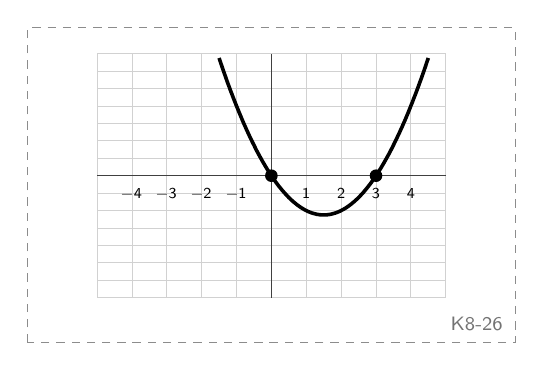
\begin{tikzpicture}
\useasboundingbox (0,0) rectangle (6.19,4.0);
\path[draw=black!18, line width=0.3pt] (0.881,0.57) -- (0.881,3.67);
\path[draw=black!18, line width=0.3pt] (1.324,0.57) -- (1.324,3.67);
\path[draw=black!18, line width=0.3pt] (1.766,0.57) -- (1.766,3.67);
\path[draw=black!18, line width=0.3pt] (2.209,0.57) -- (2.209,3.67);
\path[draw=black!18, line width=0.3pt] (2.652,0.57) -- (2.652,3.67);
\path[draw=black!18, line width=0.3pt] (3.095,0.57) -- (3.095,3.67);
\path[draw=black!18, line width=0.3pt] (3.538,0.57) -- (3.538,3.67);
\path[draw=black!18, line width=0.3pt] (3.981,0.57) -- (3.981,3.67);
\path[draw=black!18, line width=0.3pt] (4.424,0.57) -- (4.424,3.67);
\path[draw=black!18, line width=0.3pt] (4.866,0.57) -- (4.866,3.67);
\path[draw=black!18, line width=0.3pt] (5.309,0.57) -- (5.309,3.67);
\path[draw=black!18, line width=0.3pt] (0.881,0.57) -- (5.309,0.57);
\path[draw=black!18, line width=0.3pt] (0.881,0.791) -- (5.309,0.791);
\path[draw=black!18, line width=0.3pt] (0.881,1.013) -- (5.309,1.013);
\path[draw=black!18, line width=0.3pt] (0.881,1.234) -- (5.309,1.234);
\path[draw=black!18, line width=0.3pt] (0.881,1.456) -- (5.309,1.456);
\path[draw=black!18, line width=0.3pt] (0.881,1.677) -- (5.309,1.677);
\path[draw=black!18, line width=0.3pt] (0.881,1.899) -- (5.309,1.899);
\path[draw=black!18, line width=0.3pt] (0.881,2.12) -- (5.309,2.12);
\path[draw=black!18, line width=0.3pt] (0.881,2.341) -- (5.309,2.341);
\path[draw=black!18, line width=0.3pt] (0.881,2.563) -- (5.309,2.563);
\path[draw=black!18, line width=0.3pt] (0.881,2.784) -- (5.309,2.784);
\path[draw=black!18, line width=0.3pt] (0.881,3.006) -- (5.309,3.006);
\path[draw=black!18, line width=0.3pt] (0.881,3.227) -- (5.309,3.227);
\path[draw=black!18, line width=0.3pt] (0.881,3.449) -- (5.309,3.449);
\path[draw=black!18, line width=0.3pt] (0.881,3.67) -- (5.309,3.67);
\path[draw=black!75, line width=0.5pt] (0.881,2.12) -- (5.309,2.12);
\path[draw=black!75, line width=0.5pt] (3.095,0.57) -- (3.095,3.67);
\node[font=\sffamily\fontsize{5.5}{6}\selectfont, inner sep=0pt] at (1.324,1.899) {$-$4};
\node[font=\sffamily\fontsize{5.5}{6}\selectfont, inner sep=0pt] at (1.766,1.899) {$-$3};
\node[font=\sffamily\fontsize{5.5}{6}\selectfont, inner sep=0pt] at (2.209,1.899) {$-$2};
\node[font=\sffamily\fontsize{5.5}{6}\selectfont, inner sep=0pt] at (2.652,1.899) {$-$1};
\node[font=\sffamily\fontsize{5.5}{6}\selectfont, inner sep=0pt] at (3.538,1.899) {1};
\node[font=\sffamily\fontsize{5.5}{6}\selectfont, inner sep=0pt] at (3.981,1.899) {2};
\node[font=\sffamily\fontsize{5.5}{6}\selectfont, inner sep=0pt] at (4.424,1.899) {3};
\node[font=\sffamily\fontsize{5.5}{6}\selectfont, inner sep=0pt] at (4.866,1.899) {4};
\path[draw=black, line width=1.3pt] (2.431,3.615) -- (2.449,3.56) -- (2.468,3.505) -- (2.486,3.452) -- (2.505,3.399) -- (2.523,3.347) -- (2.541,3.296) -- (2.56,3.246) -- (2.578,3.196) -- (2.597,3.148) -- (2.615,3.1) -- (2.634,3.052) -- (2.652,3.006) -- (2.671,2.96) -- (2.689,2.915) -- (2.708,2.871) -- (2.726,2.827) -- (2.744,2.785) -- (2.763,2.743) -- (2.781,2.702) -- (2.8,2.661) -- (2.818,2.622) -- (2.837,2.583) -- (2.855,2.545) -- (2.874,2.508) -- (2.892,2.471) -- (2.91,2.435) -- (2.929,2.4) -- (2.947,2.366) -- (2.966,2.333) -- (2.984,2.3) -- (3.003,2.268) -- (3.021,2.237) -- (3.04,2.206) -- (3.058,2.177) -- (3.077,2.148) -- (3.095,2.12) -- (3.113,2.093) -- (3.132,2.066) -- (3.15,2.04) -- (3.169,2.015) -- (3.187,1.991) -- (3.206,1.968) -- (3.224,1.945) -- (3.243,1.923) -- (3.261,1.902) -- (3.28,1.882) -- (3.298,1.862) -- (3.316,1.843) -- (3.335,1.825) -- (3.353,1.808) -- (3.372,1.791) -- (3.39,1.776) -- (3.409,1.761) -- (3.427,1.746) -- (3.446,1.733) -- (3.464,1.72) -- (3.483,1.708) -- (3.501,1.697) -- (3.519,1.687) -- (3.538,1.677) -- (3.556,1.668) -- (3.575,1.66) -- (3.593,1.653) -- (3.612,1.646) -- (3.63,1.641) -- (3.649,1.636) -- (3.667,1.631) -- (3.685,1.628) -- (3.704,1.625) -- (3.722,1.623) -- (3.741,1.622) -- (3.759,1.622) -- (3.778,1.622) -- (3.796,1.623) -- (3.815,1.625) -- (3.833,1.628) -- (3.852,1.631) -- (3.87,1.636) -- (3.888,1.641) -- (3.907,1.646) -- (3.925,1.653) -- (3.944,1.66) -- (3.962,1.668) -- (3.981,1.677) -- (3.999,1.687) -- (4.018,1.697) -- (4.036,1.708) -- (4.055,1.72) -- (4.073,1.733) -- (4.091,1.746) -- (4.11,1.761) -- (4.128,1.776) -- (4.147,1.791) -- (4.165,1.808) -- (4.184,1.825) -- (4.202,1.843) -- (4.221,1.862) -- (4.239,1.882) -- (4.258,1.902) -- (4.276,1.923) -- (4.294,1.945) -- (4.313,1.968) -- (4.331,1.991) -- (4.35,2.015) -- (4.368,2.04) -- (4.387,2.066) -- (4.405,2.093) -- (4.424,2.12) -- (4.442,2.148) -- (4.46,2.177) -- (4.479,2.206) -- (4.497,2.237) -- (4.516,2.268) -- (4.534,2.3) -- (4.553,2.333) -- (4.571,2.366) -- (4.59,2.4) -- (4.608,2.435) -- (4.627,2.471) -- (4.645,2.508) -- (4.663,2.545) -- (4.682,2.583) -- (4.7,2.622) -- (4.719,2.661) -- (4.737,2.702) -- (4.756,2.743) -- (4.774,2.785) -- (4.793,2.827) -- (4.811,2.871) -- (4.83,2.915) -- (4.848,2.96) -- (4.866,3.006) -- (4.885,3.052) -- (4.903,3.1) -- (4.922,3.148) -- (4.94,3.196) -- (4.959,3.246) -- (4.977,3.296) -- (4.996,3.347) -- (5.014,3.399) -- (5.033,3.452) -- (5.051,3.505) -- (5.069,3.56) -- (5.088,3.615);
\path[fill=black] (3.095,2.12) circle[radius=0.08];
\path[fill=black] (4.424,2.12) circle[radius=0.08];
\draw[black!45, line width=0.4pt, dash pattern=on 3pt off 2.5pt] (0,0) rectangle (6.19,4.0);
\node[anchor=south east, font=\sffamily\scriptsize, text=black!55, inner sep=0pt] at (6.04,0.14) {K8-26};
\end{tikzpicture}%
\begin{tikzpicture}
\useasboundingbox (0,0) rectangle (6.19,4.0);
\node[text width=5.29cm, align=center, font=\Large] at (3.095,2.08) {$f(x) = x(x - 3)$};
\draw[black!45, line width=0.4pt, dash pattern=on 3pt off 2.5pt] (0,0) rectangle (6.19,4.0);
\node[anchor=south east, font=\sffamily\scriptsize, text=black!55, inner sep=0pt] at (6.04,0.14) {K8-27};
\end{tikzpicture}%
\par\nointerlineskip
\noindent\begin{tikzpicture}
\useasboundingbox (0,0) rectangle (6.19,4.0);
\node[text width=5.29cm, align=center, font=\large] at (3.095,2.08) {Nullpunkter: $x = 1$ og $x = 4$};
\draw[black!45, line width=0.4pt, dash pattern=on 3pt off 2.5pt] (0,0) rectangle (6.19,4.0);
\node[anchor=south east, font=\sffamily\scriptsize, text=black!55, inner sep=0pt] at (6.04,0.14) {K8-28};
\end{tikzpicture}%
\begin{tikzpicture}
\useasboundingbox (0,0) rectangle (6.19,4.0);
\node[anchor=south east, font=\sffamily\scriptsize, text=black!40, inner sep=0pt] at (6.04,0.14) {Eget kort};
\draw[black!45, line width=0.4pt, dash pattern=on 3pt off 2.5pt] (0,0) rectangle (6.19,4.0);
\end{tikzpicture}%
\begin{tikzpicture}
\useasboundingbox (0,0) rectangle (6.19,4.0);
\node[anchor=south east, font=\sffamily\scriptsize, text=black!40, inner sep=0pt] at (6.04,0.14) {Eget kort};
\draw[black!45, line width=0.4pt, dash pattern=on 3pt off 2.5pt] (0,0) rectangle (6.19,4.0);
\end{tikzpicture}%
\par\nointerlineskip
\noindent\begin{tikzpicture}
\useasboundingbox (0,0) rectangle (6.19,4.0);
\node[anchor=south east, font=\sffamily\scriptsize, text=black!40, inner sep=0pt] at (6.04,0.14) {Eget kort};
\draw[black!45, line width=0.4pt, dash pattern=on 3pt off 2.5pt] (0,0) rectangle (6.19,4.0);
\end{tikzpicture}%
\begin{tikzpicture}
\useasboundingbox (0,0) rectangle (6.19,4.0);
\node[anchor=south east, font=\sffamily\scriptsize, text=black!40, inner sep=0pt] at (6.04,0.14) {Eget kort};
\draw[black!45, line width=0.4pt, dash pattern=on 3pt off 2.5pt] (0,0) rectangle (6.19,4.0);
\end{tikzpicture}%
\begin{tikzpicture}
\useasboundingbox (0,0) rectangle (6.19,4.0);
\node[anchor=south east, font=\sffamily\scriptsize, text=black!40, inner sep=0pt] at (6.04,0.14) {Eget kort};
\draw[black!45, line width=0.4pt, dash pattern=on 3pt off 2.5pt] (0,0) rectangle (6.19,4.0);
\end{tikzpicture}%
\par\nointerlineskip
\end{document}
